\documentclass[letterpaper,10pt]{article}
\usepackage[utf8]{inputenc}
\usepackage{fullpage}
\usepackage[english]{babel}
\usepackage{amsmath}
\usepackage{caption}
\usepackage{subcaption}
\usepackage{graphicx}
\usepackage{amssymb}

\renewcommand{\arraystretch}{1.4}
\setlength{\parindent}{0cm}

\begin{document}

\noindent
\begin{flushright}
    \large\textbf{Miguel Alcón Doganoc} \\
    Combinatorial Problem Solving \\
    \today
\end{flushright}

\newcommand{\code}[1]{\texttt{#1}}

\noindent
{\huge{\textbf{Logic Synthesis}}}

\section{Description of the problem}
In this project, our goal is to solve the \textit{NOR Logic Synthesis Problem}
(NLSP): given a specification of a Boolean function $f(x_1,...,x_n)$ in the form of a truth table, find a NOR-circuit satisfying the specification that minimizes depth (and, in case of a tie in depth, with minimum size). An instance of NLSP consists in:
\begin{itemize}
    \item $\mathbf{n} := $ ``Number of input signals''
    \item $\mathbf{y_t} := $ ``Desired output signal, described by row $t$ in the truth table'', where $t \in \{0,1,...,2^n-1\}$  
\end{itemize}

\section{Decision variables}
Given the number of input signals $n$, the depth $d$,  the size $s$, and the truth table of the logical circuit, I defined the following variables:
\begin{itemize}
    \item $\mathbf{Z_{i,j}}:=$ ``The node ($i$,$j$) contains a constant zero'', where
    \begin{itemize}
        \item $0 \leq i \leq d$
        \item $0 \leq j < 2^i$
    \end{itemize}
    \item $\mathbf{N_{i,j}}:=$ ``The node ($i$,$j$) contains a NOR gate'', where
    \begin{itemize}
        \item $0 \leq i \leq d$
        \item $0 \leq j < 2^i$
    \end{itemize}
    \item $\mathbf{I_{i,j,k}}:=$ ``The node ($i$,$j$) contains the input $k$'', where
    \begin{itemize}
        \item $0 \leq i \leq d$
        \item $0 \leq j < 2^i$
        \item $1 \leq k \leq n$
    \end{itemize}
    \item $\mathbf{B_{i,j}^{(t)}}:=$ ``Boolean value of the node ($i,j$) for the row $t$ of the truth table'', where
    \begin{itemize}
        \item $0 \leq i \leq d$
        \item $0 \leq j < 2^i$
        \item $0 \leq t < 2^n$
    \end{itemize}
\end{itemize}

For example, for a NOR-circuit that implements the functionality of an AND gate (see figure \ref{fig:original}), with $n = d = 2$, one possible solution (variable assignation) is shown in figure \ref{fig:variables}.
\begin{figure}[hbtp]
    \centering
    \begin{subfigure}[b]{0.45\textwidth}
        \raisebox{18mm}{\begin{tabular}{c c | c | c}
            $x_1$ & $x_2$ & $y$ & $t$\\ \hline
            0 & 0 & 0 & 0 \\
            0 & 1 & 0 & 1 \\
            1 & 0 & 0 & 2 \\
            1 & 1 & 1 & 3 \\
        \end{tabular}}
    \end{subfigure}\hspace{-0.2\textwidth}
    \begin{subfigure}[b]{0.45\textwidth}
        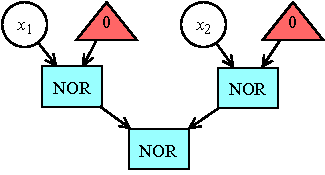
\includegraphics[width=\textwidth]{circuit.pdf}
    \end{subfigure}
    \caption{Truth table of $y$ = AND($x_1,x_2$) and NOR-circuit implementing it.}
    \label{fig:original}
\end{figure}

\begin{figure}[hbtp]
    \centering
    \begin{subfigure}[b]{0.30\textwidth}
        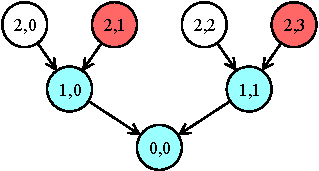
\includegraphics[width=\textwidth]{i.pdf}
        \caption{$i,j$}
        \label{subfig:i}
    \end{subfigure}
    \hspace{0.01\textwidth}
    \begin{subfigure}[b]{0.30\textwidth}
        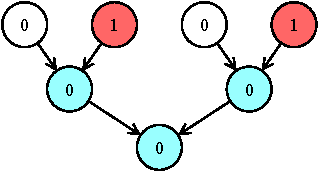
\includegraphics[width=\textwidth]{Z.pdf}
        \caption{$Z_{i,j}$}
        \label{subfig:zi}
    \end{subfigure}
    \hspace{0.01\textwidth}
    \begin{subfigure}[b]{0.30\textwidth}
        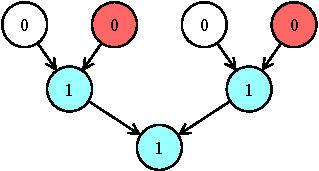
\includegraphics[width=\textwidth]{N.pdf}
        \caption{$N_{i,j}$}
        \label{subfig:ni}
    \end{subfigure}
    \begin{subfigure}[b]{0.30\textwidth}
        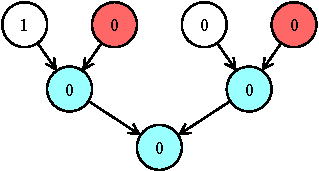
\includegraphics[width=\textwidth]{I1.pdf}
        \caption{$I_{i,j,1}$}
        \label{subfig:i1}
    \end{subfigure}
    \hspace{0.01\textwidth}
    \begin{subfigure}[b]{0.30\textwidth}
        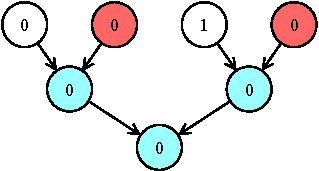
\includegraphics[width=\textwidth]{I2.pdf}
        \caption{$I_{i,j,2}$}
        \label{subfig:i2}
    \end{subfigure}
    \hspace{0.01\textwidth}
    \begin{subfigure}[b]{0.30\textwidth}
        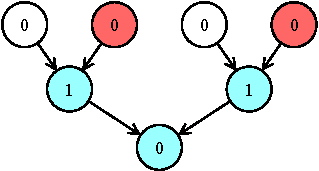
\includegraphics[width=\textwidth]{bit.pdf}
        \caption{$B_{i,j}^{(0)}$}
        \label{subfig:bit}
    \end{subfigure}
    \caption{Visual representation of ($i,j$) and the variables.}
    \label{fig:variables}
\end{figure}

\section{Constraints}
In order to simplify the definition of the constraints, I define the following functions. Given the variable $v_{i,j}$, with $v_{i,j} \in \{Z_{i,j}; N_{i,j}; I_{i,j,k}; B_{i,j}^{(t)}\}$,
\begin{itemize}
    \item \textbf{left($v_{i,j}$)} := ``Variable corresponding to the one on the left of $v_{i,j}$'' $ \equiv v_{i+1,2\times j}$.
    \item \textbf{right($v_{i,j}$)} := ``Variable corresponding to the one on the right of $v_{i,j}$'' $ \equiv v_{i+1,2\times j+1}$.
    \item \textbf{bit($k,t$)} := ``Boolean value of $x_k$ in the $t$-th row of the truth table'' $\equiv$ ``Value of the position $k$ of the binary representation of $t$ (i.e. $t_k \in \{t_1 t_2 ... t_n$\})''.
    \item  \textbf{AMO($l$)} := ``Given the list of variables $l$, at most one of the variables in it can be true.'' %$\equiv$ If $l = \{x_0,...,x_m-1\}$:
    % \begin{align*}
    %     \lnot x_i \lor \lnot x_j \\
    %     \forall 0 \leq i < j < n
    % \end{align*}
    \item \textbf{AMK($k; l$)} := ``Given the list of variables $l$, at most $k$ of the variables in it can be true.''
\end{itemize}
I defined \textbf{AMO} and \textbf{AMK} as it is explained in the SAT encoding slides. The constraints that define the problem are the following:
\begin{itemize}
    \item The output of the circuit is equal to the desired value for each row $t$ of the truth table.
    \begin{align*}
        \text{if }y_t\text{ then }B_{0,0}^{(t)} \\
        \text{otherwise }\lnot B_{0,0}^{(t)} \\
        \forall t < 2^n
    \end{align*}
    \item NOR gates are not allowed on the leaves of the circuit.
    \begin{align*}
        \lnot N_{d,j} \\
        \forall j < 2^d 
    \end{align*}
    \item Force children (if any) of each node to be 0 if the node is not a NOR gate.
    \begin{align*}
        N_{i,j} \lor \mathbf{left}(Z_{i,j}) \\
        N_{i,j} \lor \mathbf{right}(Z_{i,j}) \\
        \forall i < d\text{ }\forall j < 2^i
    \end{align*}
    \item Link each NOR gate with its corresponding value, which is the NOR operation between both children.
    \begin{align*}
        \lnot N_{i,j} \lor \lnot \mathbf{left}(B_{i,j}^{(t)}) \lor \lnot B_{i,j}^{(t)} \\
        \lnot N_{i,j} \lor \lnot \mathbf{right}(B_{i,j}^{(t)}) \lor \lnot B_{i,j}^{(t)} \\
        \lnot N_{i,j} \lor \mathbf{left}(B_{i,j}^{(t)}) \lor \mathbf{right}(B_{i,j}^{(t)}) \lor B_{i,j}^{(t)} \\
        \forall t < 2^n\text{ }\forall i < d\text{ }\forall j < 2^i
    \end{align*}
    \item Link each constant 0 signal with `false'.
    \begin{align*}
        \lnot Z_{i,j}  \lor \lnot B_{i,j}^{(t)} \\
        \forall t < 2^n\text{ }\forall i \leq d\text{ }\forall j < 2^i
    \end{align*}
    \item Link each input signal that has value 1 in the truth table, with `true'.
    \begin{align*}
        \text{if }\mathbf{bit}(k,t)\text{ then }\lnot I_{i,j,k} \lor B_{i,j}^{(t)} \\
        \text{otherwise }\lnot I_{i,j,k} \lor \lnot B_{i,j}^{(t)} \\
        \forall 1 \leq k \leq n\text{ }\forall t  < 2^n\text{ }\forall i \leq d\text{ }\forall j < 2^i
    \end{align*}
    \item Force each node to be only of one type.
    \begin{align*}
        \mathbf{AMO}(\{Z_{i,j}, N_{i,j}, I_{i,j,1}, I_{i,j,2}, ..., I_{i,j,n}\})\\
        Z_{i,j} \lor N_{i,j} \lor I_{i,j,1} \lor I_{i,j,2} \lor ... \lor I_{i,j,n}\\
        \forall i < d\text{ }\forall j < 2^i
    \end{align*}
    \item Limit the number of NOR gates to be less than size.
    \begin{align*}
        \mathbf{AMK}(s; \{Z_{i,j}, N_{i,j}, I_{i,j,1}, I_{i,j,2}, ..., I_{i,j,n}\})\\
        Z_{i,j} \lor N_{i,j} \lor I_{i,j,1} \lor I_{i,j,2} \lor ... \lor I_{i,j,n}\\
        \forall i < d\text{ }\forall j < 2^i
    \end{align*}
\end{itemize}

\subsection{Worsen performance}
I tried to use some constraints that at the end affected negatively to the performance of the program.
\begin{itemize}
\item Force non-symmetry of NOR gates' children.
\begin{itemize}
    \item Do not allow the same input on both sides.
        \begin{align*}
            \mathbf{AMO}(\{\mathbf{left}(I_{i,j,k}), \mathbf{right}(I_{i,j,k})\}) \\
            \forall i < d\text{ }\forall j < 2^i\text{ }\forall k \leq n
        \end{align*}
\end{itemize}
\end{itemize}

\section{Extra comments}
I tried two implementations of \textbf{AMO}, the quadratic and logarithmic encodings. At the final version of the program, I used the quadratic one because I had better performance with it. Both encodings are implemented in the program, but the logarithmic one is not used. 

I also used the \code{frozenset} of \textit{Python} to avoid repeating clauses and variables inside the clauses.

The program is able to solve all the problems in 511s. With 1 min of \code{timeout}, it never has to stop the program because it finished its execution before. Inside the `out/' directory you can find the solutions for to problems.

\end{document}